\chapter{\hlc[red]{Rio de Janeiro Mangroves}} \label{ch:mangroves}



\section{\hlc[yellow]{Study Area \& Context}}

Guaratiba is a relatively rural district of Rio de Janeiro situated in the southwestern corner of the municipality. It is home to a mix of land uses, including decorative plant farming, multiple fishing communities, a military base and training center, a state-run biological reserve, some informal settlements, and a growing ecotourism industry. The biological reserve exists to protect the largest remaining mangrove forest within the municipality. These mangroves are vulnerable due to landward urbanization, including a recently opened urban transit line, and rising sea levels \cite{goldbergEcoMapDecisionsupportTool2018} They provide a variety of ecosystem services, including serving as a mechanism for highly efficient carbon sequestration, supporting a small-scale industry of fishing and crab catching, preventing coastal erosion, and attracting the aforementioned local ecotourism industry \cite{schwenkResearchEnvironmentalSocioeconomical2008}. Government policies to conserve the mangroves can use integrated modeling tools to consider both the benefits of protecting the forests as well as the economic needs of low-income communities. This, coupled with the Rio de Janeiro municipal government's pre-existing interest in generating useful datasets and making them available online through the Data.Rio platform \cite{matheusOpenGovernmentData2014}, made the Guaratiba mangroves a particularly suitable case study for the \ac{evdt} Modeling Framework.

Our primary Local Context Experts and points of contact are at \ac{ipp}, which is the municipal data agency, and ESPAÇO, a research group at the \ac{ufrj} who study various coastal ecosystems in Brazil and elsewhere \cite{cruzClassificacaoOrientadaObjetos2007, seabraMapeamentoDinamicaCobertura2013} and who are also familiar with examining socioeconomic impacts of environmental phenomena \cite{schwenkResearchEnvironmentalSocioeconomical2008}. The latter can also be considered to be Technical Area Experts. Other Local Context Experts include a member of a local fisher association and government officials at the municipal urban development agency and the municipal environmental agency Additional Technical Area Experts include two ecosystem services economists (one from the University of West Virginia and one from \ac{rff}) and arguably the committee members for this thesis. The primary intended users for this case study are government officials at the \ac{ipp} who have a fair amount of experience with mapping. Future projects in this area would ideally expand that userbase to non-government individuals. 

This project began in 2018 and since that time Jack Reid made two multi-week field visits to Rio de Janeiro and Guaratiba in particular.

\subsection{\hlc[red]{Stakeholders}}

a

\section{\hlc[red]{Systems Architecture Framework}}

a

\subsection{\hlc[red]{Interviews}}

a

\begin{figure}[h]
	\centering
	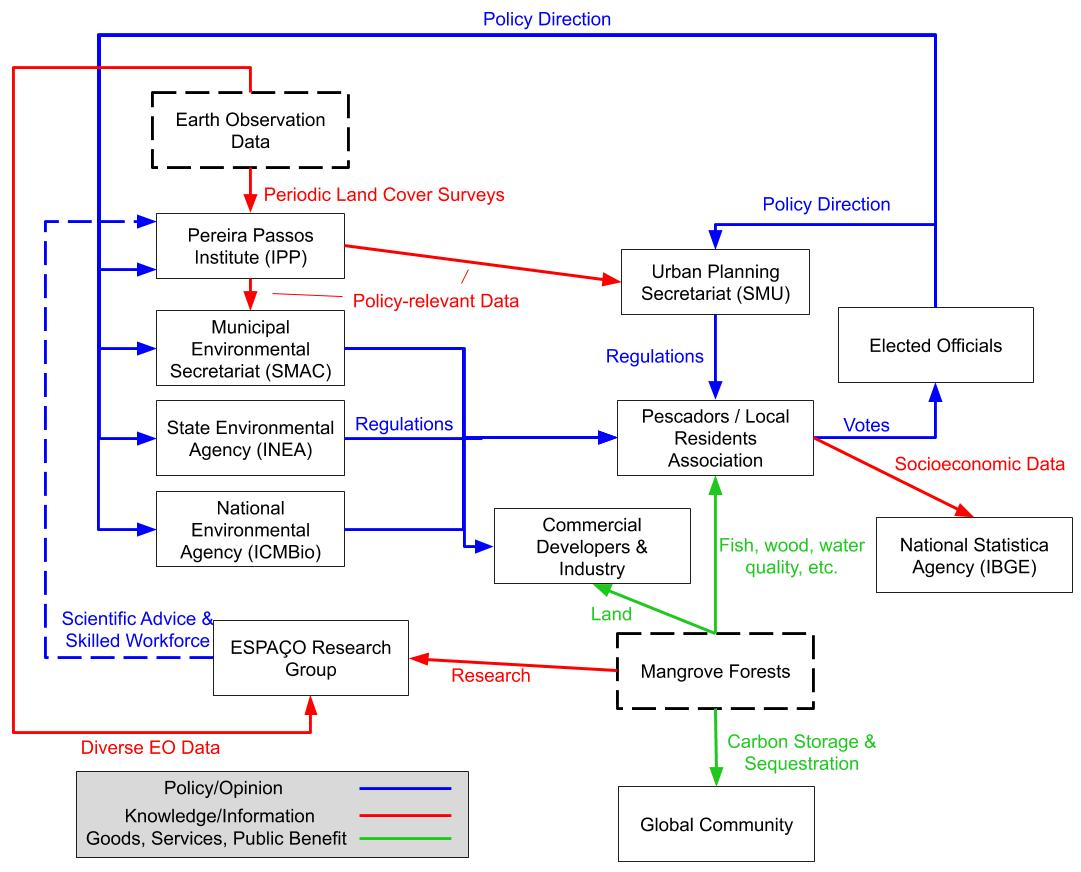
\includegraphics[scale=0.3]{Figures/chap4/Stakeholder_Map_v2.jpg}
	\caption[Stakeholder Map for the Mangrove Forests of Rio de Janeiro]{Stakeholder Map for the Mangrove Forests of Rio de Janeiro}
	\label{fig:rio_stakemap}
\end{figure}

\subsection{\hlc[red]{Needs, Outcomes, and Objectives}}

a

\subsection{\hlc[red]{System Architecture}}


\section{\hlc[red]{EVDT Application}}

\subsection{\hlc[red]{Environment:}}

\subsection{\hlc[red]{Vulnerability}}

\subsection{\hlc[red]{Decision-making}}

\subsection{\hlc[red]{Technology}}

\section{\hlc[red]{Decision Support System}}

\section{\hlc[red]{Evaluation}}

\section{\hlc[red]{Discussion}}





